All simulations were ran with the same fixed NFW profile with the following parameters:
\begin{itemize}
    \item $c = 20.1$
    \item $R = 16.1$ kpc
    \item $M_{H} = 1.53 \times 10^{12}$ $\msun$,
\end{itemize}
where $c$ is the concentration parameter such that
$$
    M_{H} = 4\pi \rho_{DM} R^3 \left[ \ln (1 + c) - \frac{c}{1+c} \right]~,
$$
is the mass of the halo with $R$ the scale radius.
The density of the halo as a function of radius is 
\begin{equation}
    \rho(r) = \frac{\rho_{DM}}{\frac{r}{R} \left( 1 + \frac{r}{R} \right)^2}~,
    \label{eqn:nfw}
\end{equation}
the NFW profile.

The runs also have a fixed total mass in the disk, of $8\times10^{10} \msun$ to reproduce approximately the mass of the Milky Way.
The disks are initialised with an exponential profile, with scale radius $3$ kpc for both stellar and gaseous material.
The scale height of the gas is initialised to be 2 kpc, with the stellar component initially having a scale height of 0.3 kpc.

\subsection{Resolution Dependence}

The simulations are shown after $\approx 2$ Gyr of evolution in Figure \ref{fig:sdbig}. At first glance, the simulations appear to be approximately resolution-independent, relaxing to a similar disk relatively quickly.

Of particular interest is the scale height of the disk between the {\tt custom\_lowres}, {\tt custom}, and {\tt custom\_highres} runs.
These are calculated by fitting an exponential profile,
$$
    ACTUAL EQUATION
$$
and the results are shown in Figure \ref{fig:vheighthist}.

\begin{figure}
    \centering
    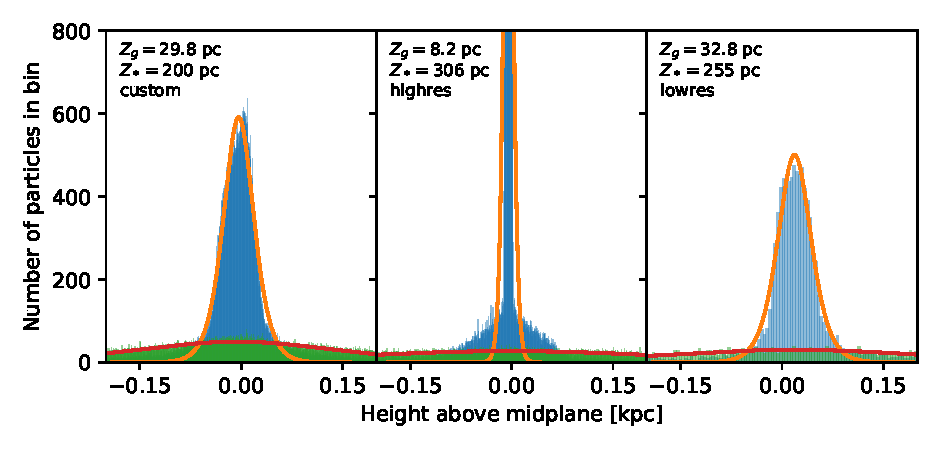
\includegraphics{v_height_hist.pdf}
    \caption{The vertical distribution of the particles in the disk (for {\tt custom}, {\tt custom\_highres} and {\tt custom\_lowres}) after $\approx 2$ Gyr of evolution from the initial conditions. The top set of histograms encompasses all of the data, whereas the bottom set exclude the particles residing within the inner $0.5$ kpc of the galaxy. In blue and orange, the gas histogram and fit are shown, with the same for the star particles being shown in green and red. The fits use the density profile in Equation \ref{eqn:vertprofile}, with $Z_g$ the scale height of the gas and $Z_*$ the scale height of the stellar disk. The {\tt custom\_lowres} is shown with bins ten times as wide as to normalise the overall contents of the histogram. It appears that the scale height of the gas disk is determined by the chosen softening length, as the {\tt custom\_highres} run has a considerable build up of particles within the very centre of the disk. Normally, the disk is spread vertically by the ejection from supernovae explosions, and as these are not modelled in a local way in the {\tt custom} model a high degree of clumping is shown. From the splitting of the histograms, it is clear that there are two regimes here; the inner $\approx 0.5$ kpc, and the rest of the galaxy. The inner region (see Figure \ref{fig::sd_r}) contains the majority of the mass in the galaxy, and as such the gaseous disk is highly compressed (the {\tt custom\_highres} run shows this in most detail because of the smaller gravitational softening). This suggests that the model presented in this work does not account for all of the dynamics in the galaxy, which is to be expected as there are several key components missing (see \S \ref{sec:missing}).}
    \label{fig:vheighthist}
\end{figure}

\begin{figure}[!ht]
    \savebox{\graphicsbox}{\includegraphics[trim={1.95cm 1.9cm 1.9cm 1.9cm}]{sd_simulation.pdf}}% Store image
    \leavevmode\rlap{\usebox{\graphicsbox}}% Set image with complete overlap
    \begin{minipage}[b]{0.63\wd\graphicsbox}% Insert caption
        \caption{The surface density (in gas only) of each of the runs from Table \ref{tab:sims} is shown, with colour encoding surface density. Note that the colour map is cut off below $0.1 \msun \pc^{-2}$ and above $1000 \msun \pc^{-2}$ for clarity. Spiral structure has formed in the {\tt custom} runs with density waves permeating the whole galaxy, whereas the {\tt default} runs have remained relatively uniform.}
        \label{fig:sdbig}
    \end{minipage}\hspace*{0.33\wd\graphicsbox}% Add space to represent figure width
\end{figure}


